\documentclass[12pt]{article}
 
\usepackage[margin=1in]{geometry} 
\usepackage{amsmath,amsthm,amssymb}
\usepackage[margin=1in]{geometry} 
\usepackage{amsmath,amsthm,amssymb}
\usepackage[T1]{fontenc}
\usepackage[utf8]{inputenc}
\usepackage{lmodern}
\usepackage{graphicx}
\usepackage{hyperref}

\newenvironment{solution}{\begin{proof}[Solution]}{\end{proof}}
 
\begin{document}
 
\title{Comparing Airbnb Listings and Housing Rental Markets in New York City}
\author{Cameron Cabo\\
ccabo@seas.upenn.edu}

\maketitle
\section{Motivations}

New York City is often a leader and outlier. Sadly, this holds true as much today, amidst the Coronavirus outbreak, as it ever has. New York are also a leader in regulation, markets, and pushing the agenda (for example, mandating that Airbnb and similar platforms share data with the government\footnote{https://www.wired.com/story/airbnb-new-york-city-reach-truce-on-home-sharing-data/}). Thus analyzing the data in New York, specifically, can be a useful indicator for how other municipalities can deal with their own housing problems and to understand how technology has real-world impacts on real-world systems.

More personally, I've done a good amount of research into the impacts rideshare companies like Uber and Lyft have on traffic patterns, equality, and on transit ridership and investment.\footnote{https://www.cameroncabo.com/thoughts/classism-in-the-gig-economy} More recently, I've looked into how alternative ownership structures like land trusts and cooperatives can solve problems with inequality in cities. Closely related to both of these problems is analyzing the impact Airbnb and related short term rental platforms have on communities in cities.

\section{Data Overview}

\subsection{Inside Airbnb NYC Listing Data}

Inside Airbnb\footnote{http://insideairbnb.com/get-the-data.html} is a website run by Murray Cox\footnote{https://twitter.com/murrayscox} which scrapes Airbnb listing data for cities around the world. The data contains almost all of the information which one can glean from looking at a listing on the Airbnb website in addition to information about the listing's host, namely how many other listings they operate and when they joined Airbnb.

This data was scraped in April, 2020.

\subsection{Scraped Inside Airbnb Neighborhood Data}

Inside Airbnb does not provide its aggregated data in a downloadable form as it does for its normal listing data. One advantage of the aggregated data is that Inside Airbnb has a model for tracking and predicting how often Airbnb listings are booked over time. They can use this to predict how much revenue a host makes per month.\footnote{http://insideairbnb.com/about.html} This makes it easier to compare Airbnb listings with more traditional rental listings in the city and to understand why a property owner would decide to list on Airbnb versus rent their property.

To access this data, I wrote a simple JavaScript which runs in the browser console to scrape this data from the website and write it to a CSV string.\footnote{https://github.com/cacabo/airbnb-nyc-data-analysis/blob/master/scrape.js}

This data was scraped in April, 2020.

\subsection{NYC Geospatial Data}

This is GeoJSON data for all boroughs (neighborhood groups) and neighborhoods in New York City provided by Inside Airbnb to make plotting the Listings data more convenient.
\footnote{http://insideairbnb.com/get-the-data.html} There are 233 neighborhoods and 5 boroughs in the dataset.

\subsection{StreetEasy NYC Rental Data}

StreetEasy is a data aggregator for rentals and housing sales. They offer up some of their data in the open domain via their website.\footnote{https://streeteasy.com/blog/data-dashboard} For this project, I looked at the rental inventory in a given neighborhood and the average asking price for rental properties in a given neighborhood. The asking price is a proxy (slightly above) the price residents likely pay for rentals already.

This data was scraped in March, 2020.

\subsection{Housing NYC Projects Data}

This dataset is provided via NYC's OpenData initiative.\footnote{https://data.cityofnewyork.us/Housing-Development/Housing-New-York-Units-by-Building/hg8x-zxpr} The dataset contains projects began in 2014 or later which are part of the Housing New York plan enacted by Mayor Bill de Blasio to ``create and preserve 200,000 high-quality, affordable homes over ten years."\footnote{https://www1.nyc.gov/site/housing/index.page} Thus, these data points provide a window into where and how much the city is investing in affordable housing for lower income groups.

The dataset breaks down the location of each project, when it occurred, various identifiers, and the breakdown of units by intended income group (extremely low income, very low income, low income, etc.).

\section{Data Engineering}

\subsection{Merging and Formatting}

First, I renamed columns from the various datasets to have common naming conventions and to use similar, convenient types (like numbers for dollar values).

Next, I joined the StreetEasy rental data with the neighborhood data from Inside Airbnb and the scraped data to aggregate all neighborhood-level data points into a single data set. Fortunately, the data sets use similar naming conventions for neighborhoods in the city which enabled a clean merge on all neighborhoods with at least two listings or housing projects (there are some outliers to the far exterior of NYC which were missing in at least one data set, but none are large Airbnb or rental markets).

I performed a spatial join on the Housing NYC data to partition the building projects into their respective neighborhoods as specified by the Inside Airbnb GeoJSON data.

\subsection{Filtering and Focusing Listings}

A major challenge was filtering this data such that the listings are actually representative of the listing market in NYC and of properties which could be used as more traditional rentals. There are 50378 unfiltered listings in the NYC Inside Airbnb dataset. I filtered the listings down to 36294 more relevant listings as follows:

\begin{itemize}
  \item Only include listings of private rooms, entire homes, or entire apartments.
  \item Each listing must be in an apartment building, house, townhouse, condo, loft, guest suite, or serviced apartment to exclude more exotic venues which could likely not serve as a traditional rental listing.
  \item Remove listings which were extremely costly on a nightly or monthly basis relative to other listings.
  \item Remove listings which accommodate enough people to, according to sampling the data, be more likely to be a venue than an apartment.
  \item Remove listings with more than eight beds. Note that many listings in the dataset of ``0'' or ``NA'' beds. Looking at samples of the data these at least appear to be legitimate listings.
  \item Remove listings which have been reviewed, but not in the past year. Many listings have never been reviewed, but still appear to be legitimate so I kept these in the data.
\end{itemize}

\subsection{Shortcomings in the Data}

Airbnb has not collaborated much with municipalities in releasing data. Moreover, it has made it more difficult over time to assess the occupancy rate of listings and does not publicize information like how much money hosts make. This forces us to make some guess work and to use variables as indicators of trends rather than sources of truth. As such, we can certainly deduce trends from the data though should hold back from making any quantitative conclusions.

Ideally, cities could reach agreements with technology companies of this nature to release data when it has large impacts on markets which the government plays a large, interventionist role in. For example, the government spends large sums of money and effort creating affordable housing or subsidizing transit. It could likely make smarter budgeting and allocation decisions with more data from Airbnb. Likewise, the government spends large sums of money maintaining and expanding transit services. It would likely make smarter budgeting and allocation decisions with more data from Uber and Lyft.

\section{Analysis}

\subsection{Impact of ``Commercial'' Hosts on Airbnb Listing Markets}

Research in this space often seeks to draw a line between ``commercial'' hosts and traditional hosts based on the scale and frequency of their operations. I wanted to better understand how different hosts take advantage of the Airbnb platform, potentially to the disadvantage of NYC residents or traditional, single-listing hosts. There are a similar number of listings in the filtered data set operated by multi-listing hosts and single-listing hosts, and there is no clear pricing or availability difference between the two sets of listings.

Differences likely would arise if we had the data behind costs incurred by hosts. In all likelihood, hosts owning multiple listings (and especially agencies owning hundreds of lisitngs) can streamline their operations and operate at lower costs. Many hosts have several listings that are located close to each other, indicating that this would be the case.

\subsection{Overlaying Airbnb Listings and Housing NYC Data}

Airbnb listings and Housing NYC Project developments tend to be in different locations in the city. Housing NYC Projects are often clustered where the city invests in rows of buildings with low cost housing units. Such properties are seldom listed on Airbnb, likely for both legal and financial reasons.

Airbnb listings are likely common in areas travellers and business people frequent: transit, shopping, and restaurant hubs. Housing NYC projects are more likely to be located in areas where rental prices grow at more steady rates even without rent controls so that the city and landlords take on a smaller opportunity cost for running these programs.

\newpage

\begin{center}
  \textbf{Housing Projects and Listings in Manhattan}

  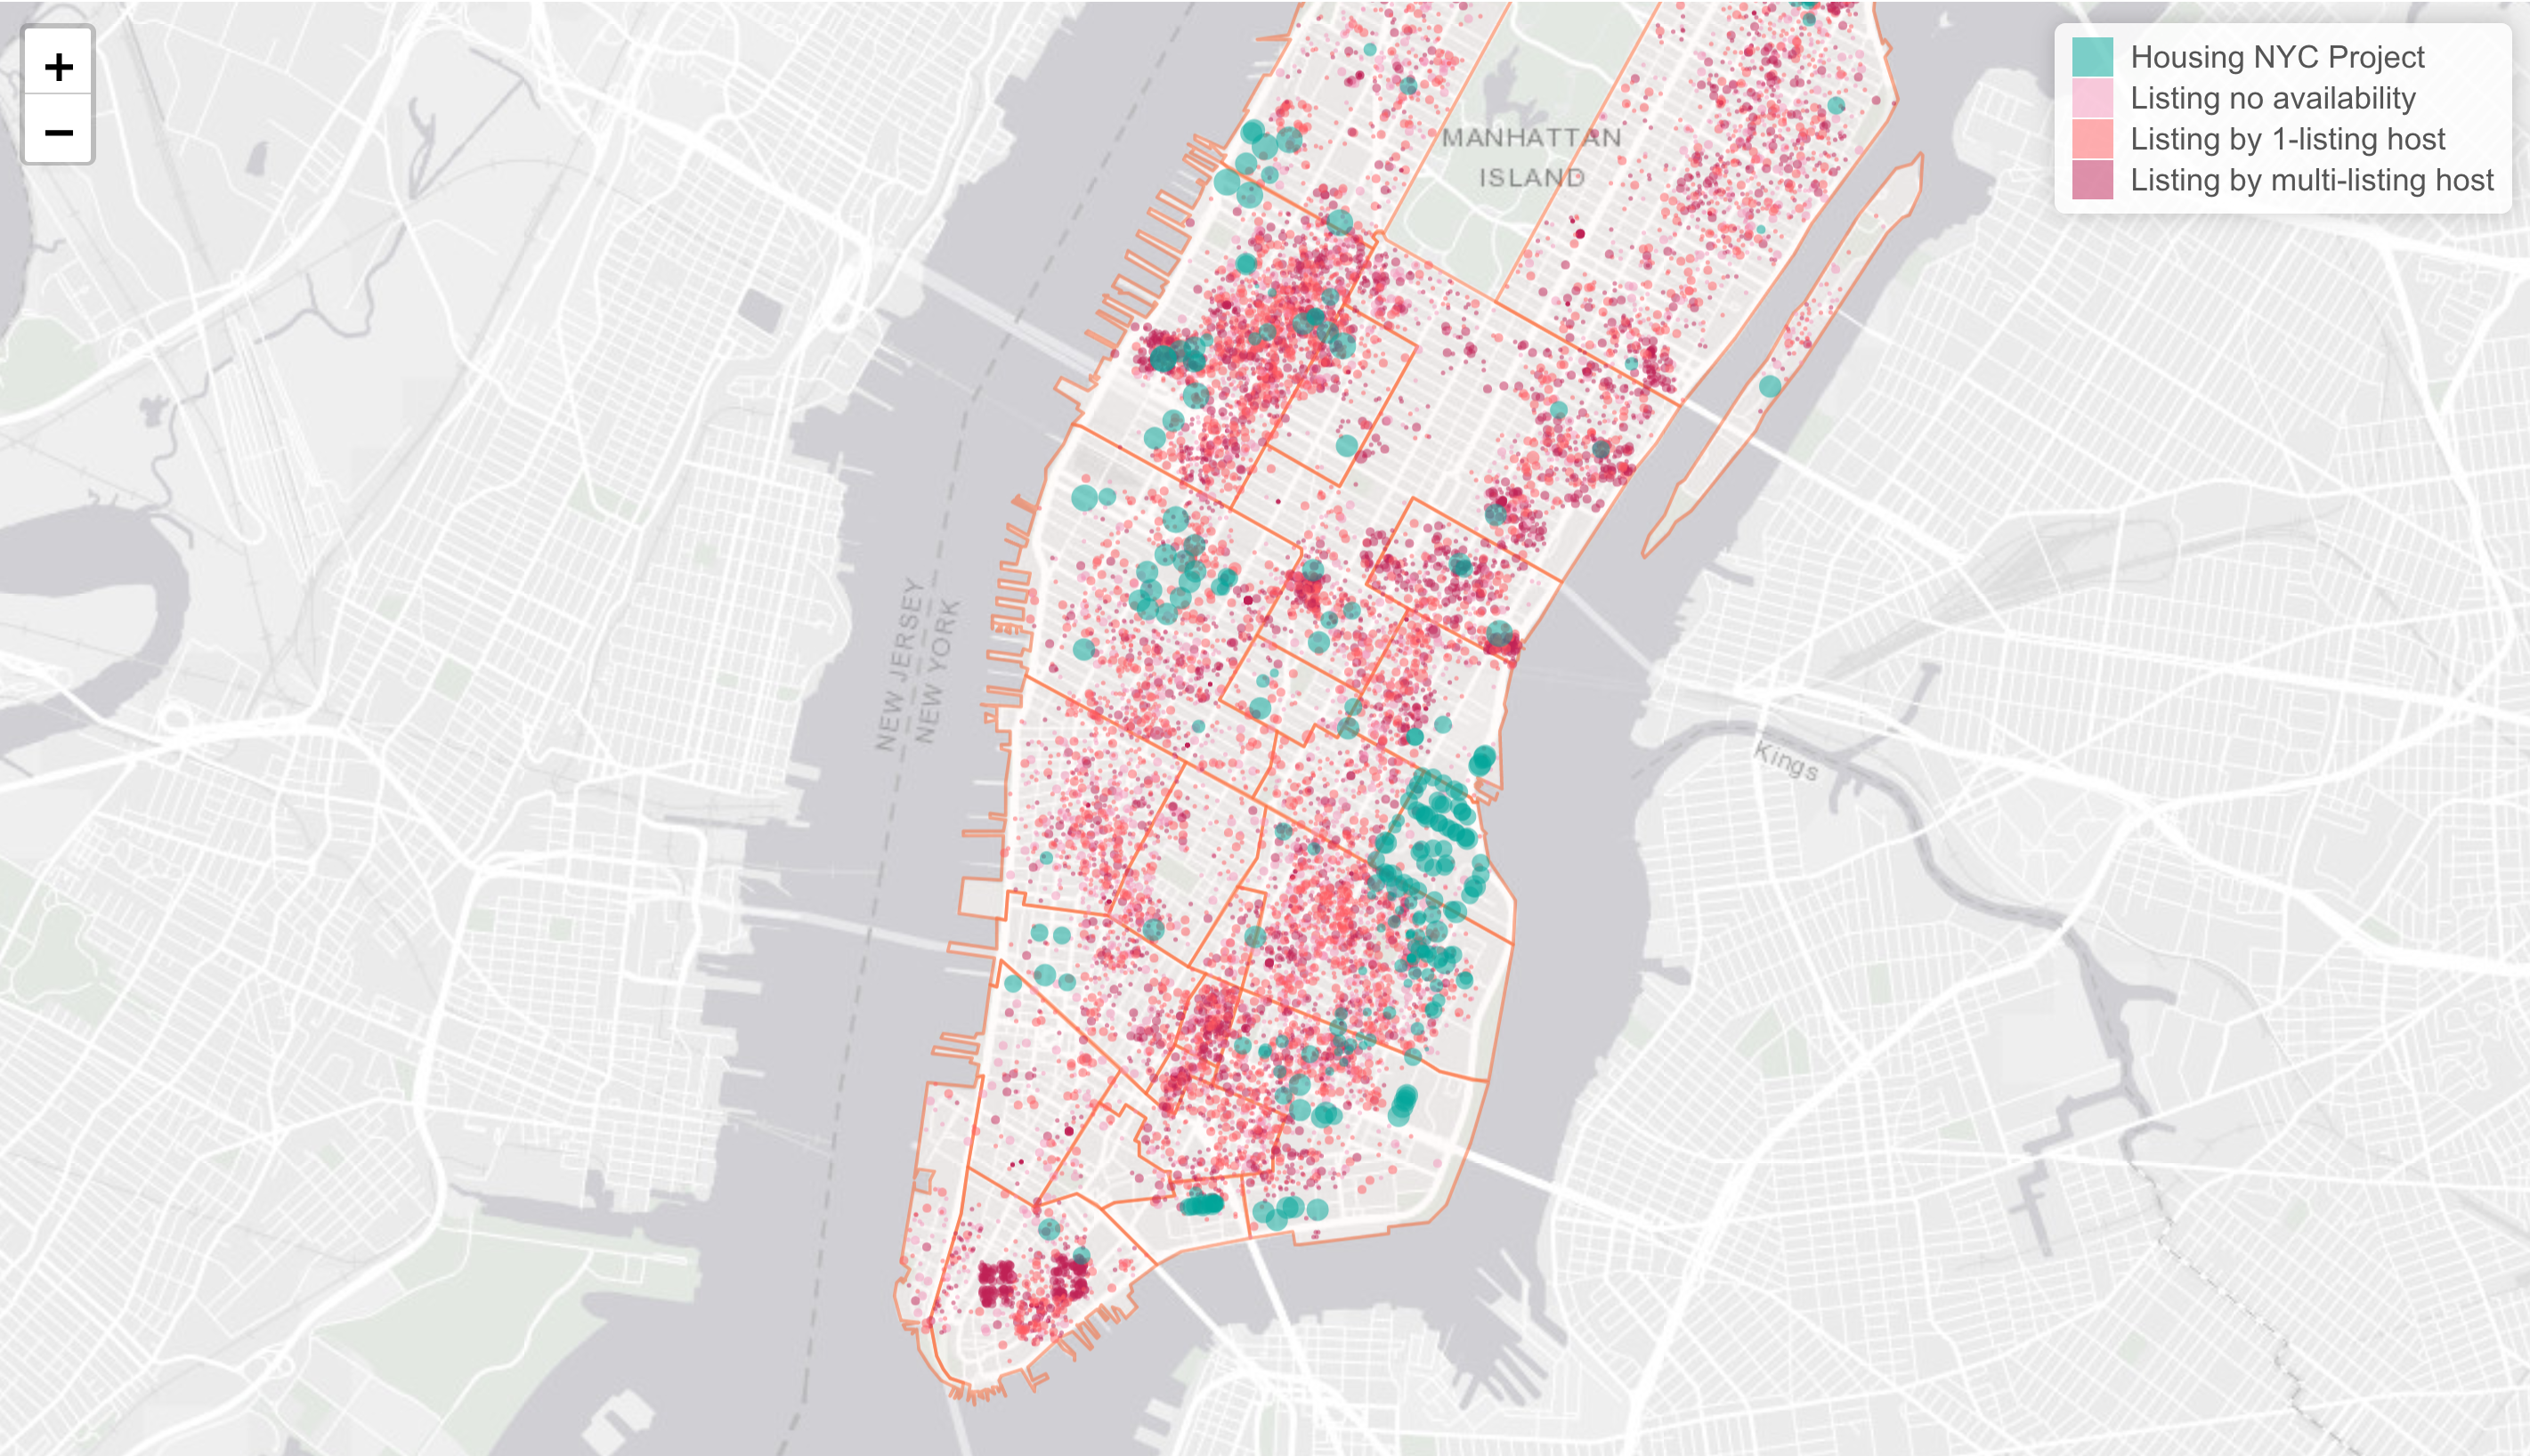
\includegraphics[width=6.5in]{./manhattan.png}
\end{center}

\begin{center}
  \textbf{Housing Projects and Listings in Brooklyn}

  \includegraphics[width=6.5in]{./brooklyn.png}
\end{center}

\newpage

\subsection{Comparing Airbnb Data and NYC Rental Data at the Neighborhood Level}

Airbnb listings are more expensive and more common in neighborhoods with higher rental prices. The causal link is hard to establish, but increasing rent prices and Airbnb concentration can have large impacts on neighborhoods and communities. Research has found vacancy rates (the percentage of rental properties without anyone living in them) for cheaper housing are far lower in NYC than for more expensive units, making it harder for lower income residents to access rental properties.

My analysis confirms this trend: there is a relatively strong correlation between monthly rental asking price and expected average Airbnb listing income (~0.76). There is a weaker correlation (~0.52) between rental inventory and expected average Airbnb listing income.

\begin{center}
  \textbf{Avg. Estimated Airbnb Income per Month by Neighborhood}

  \includegraphics[width=6.5in]{./airbnb-income.png}
\end{center}

\newpage

\begin{center}
  \textbf{Avg. Rent Asking Price by Neighborhood}

  \includegraphics[width=6.5in]{./rent-asking.png}
\end{center}

\begin{center}
  \textbf{Rent Inventory by Neighborhood}

  \includegraphics[width=6.5in]{./rent-inventory.png}
\end{center}

\newpage

\section{Recommendations}

NYC has instituted rent control\footnote{https://en.wikipedia.org/wiki/Rent\_control\_in\_New\_York} widely across the city. One issue with rent control is that it fails to align incentives between landlords and renters, leading to poor service and degrading housing conditions in the long term.\footnote{https://www.youtube.com/watch?v=oJvTTGOHFkU}

Alternatively, cooperatives can be a powerful mechanism for keeping rent low in certain localities while aligning incentives between ownership groups and those living on the property. We need stronger, more deliberate partnerships between municipal governments and these community-based organizations to redistribute earnings and wellbeing more directly. Airbnb automates the process of listing properties and disrupting markets on the higher end, though it is very hard for governments and organizations to operate at similar scale and agility at the lower end of markets.

Airbnb listings further restrict housing supply. If all Airbnb's in our dataset became rental properties, the vacancy rate in the City across the board would be at a healthier level. However, people are listing their properties on Airbnb for a reason, be it financial, professional, or social. Instead of the City limiting the number of listings and interfering with market dynamics, I think it would better align incentives to have Airbnb hosts to register with the city and pay a tax on all earnings. This tax revenue could be directly funnelled into growing alternative forms of ownership like cooperatives and land trusts beyond the scale that Housing NYC has been able to operate at. New Jersey City has such a tax in the works.\footnote{https://therealdeal.com/2015/10/12/jersey-city-mayor-wants-to-legalize-airbnb/}

Such a strategy would give the city and organizations the flexibility to invest in neighborhoods they think are the most in need for better low cost housing options and will make regulations easy to enforce across the board compared to complex licensing and permit agreements. Rather than letting Airbnb fundamentally change the dynamics of certain neighborhoods while others are bolstered with affordable housing, an income sharing model could enable more steady growth which better accommodate the needs of existing residents unable to weather increases in their rent.
 
\end{document}